\documentclass[a4paper,11pt]{article}
\usepackage[T1]{fontenc}
\usepackage[utf8]{inputenc}
\usepackage{lmodern}
% \usepackage{hyperref} % fucking warnings
\usepackage{graphicx}
\usepackage{graphics}
\usepackage{rotating}
\usepackage{listings}
\usepackage{color}
\usepackage{listings}
\usepackage{amsthm}
\usepackage{amsmath}
\usepackage{amssymb}
\usepackage{algorithmic}
\usepackage{datatool}
\usepackage{caption}
\usepackage{subcaption}

% \newcommand{\encode}[1] {{ {}_{\llcorner}{#1}_{\lrcorner}}}

\title{Numerical Linear Algebra (CSE-6643) - Final take home exam}
\author{Arash Rouhani (rarash@gatech.edu) - gtid: 902951864}


\begin{document}

\maketitle

\section{Part I}

% This task consists of (1) discretizing a differential equation into
% linear equation, (2) solving the linear equation using own
% written gauss elimination and (3) plotting,  timing and commenting on
% results.

\subsection{Discretization (exactly as previous project)}

For $n$ interior points we have $m=n+1$ interior slices. We define $h$
to $1/m$ which is the distance between the points. With this a natural
discretization appears

\[
  u''[i] = \frac{1}{2} - \frac{i}{m} = \frac{u[i+1]-2u[i]+u[i-1]}{h^2}
\]

Where $u$ is unknown, of course, we want to solve for it since it's a
differential equation. More precisely, $u[0]=u[m]=0$ are corresponding
to the given initial values and $u[i]$ exists for $i = 1..n$.

Now we want to form the typical equation $Ax=b$ such that solving for
$x$ gives all $u[i]$. The equation above gives us this scheme: Let $A$
be a tridiagonal matrix with only $-2$ in the diagonal and $1$ in its
sub- and super diagonal. Set $b_i$ to $(1/2-i*h)h^2$. $x_i$ is simply
$u[i]$ in this scheme.

\section{Part II}

\subsection{Discretization}

We note that $b$ and $x$ of our $Ax=b$ discretization are just like for
Part I.  However, $A$ is somewhat different. To construct a first we
note these equations.

\[
  u[i] = u[i]
\]
\[
  u'[i] = \frac{u[i+1]-u[i-1]}{2h}
\]
\[
  u''[i] = \frac{u[i+1]-2u[i]+u[i-1]}{h^2}
\]

The differential equation's LHS is just a linear combination of these
three kinds of variables which all can be expressed in $u[i]$ and can
hence be factored out to be the $x$ part of $Ax=b$. To actually
construct $A$ is now doable, it's just the sum of three matrices
corresponding for the three terms $u[i]$, $u'[i]$ and $u''[i]$. $A$ will
again be tridiagonal. The diagonal will be affected by the $u[i]$ term
and the $u''[i]$ term while the two outer diagonals will be affected by
$u'[i]$ term and again the $u''[i]$ term. For matrix term corresponding
to the $u[i]$ part is $\lambda*I$ where $I$ is the $n$ by $n$ identity
matrix.

\subsection{The Positive Definite Constraint}

A requirement for both Steepest descent and conjugate gradient is that
the matrix $A$ in $Ax=b$ is Positive definite. I checked by construction
that all matrices are positive definite, so luckily it doesn't impose
any problem. If it however would pose a problem, one could always solve
the system $A^{*}Ax=A^{*}b$ since $A^*A$ is always positive definite and
gets carried out in $O(1)$ for tridiagonal $A$.










\subsection{Example pic!}

\begin{figure}
        \begin{subfigure}[b]{1.0\textwidth}
          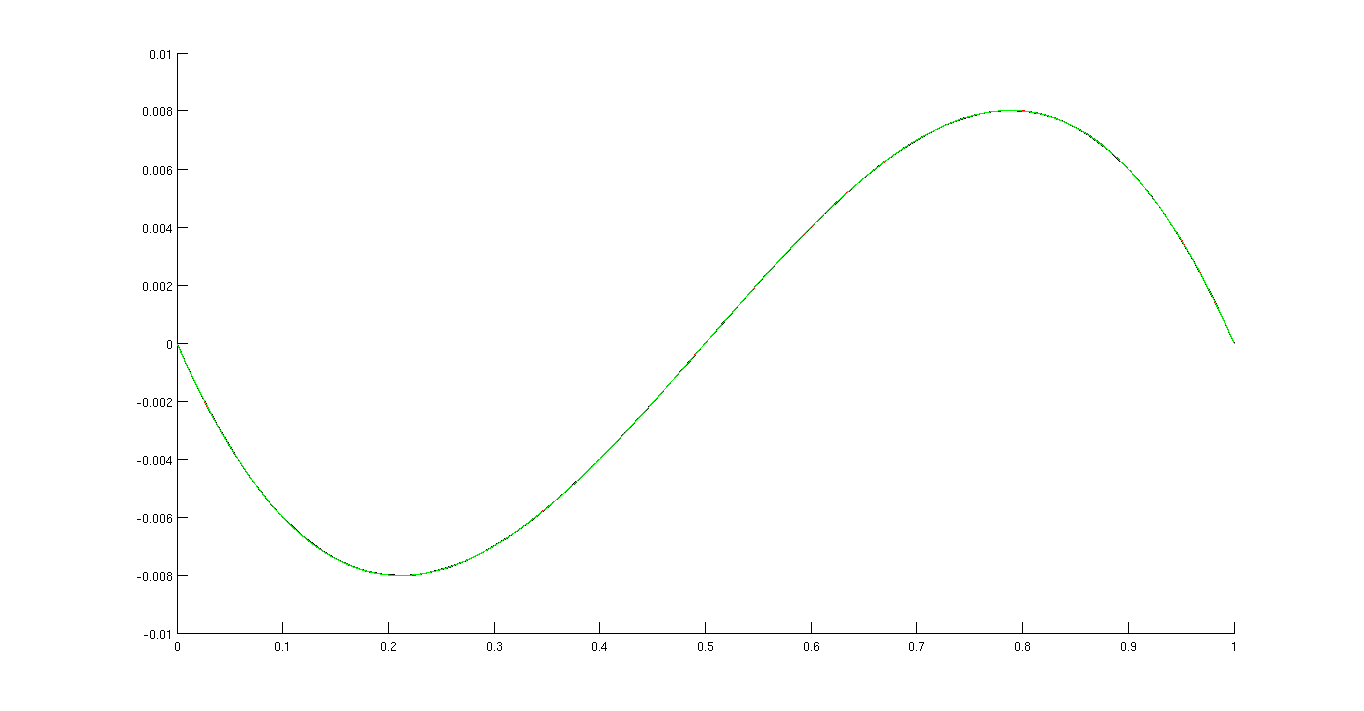
\includegraphics[width=\textwidth]{fig/all.png}
          \caption{The whole plot}\label{fig:wholeplot}
        \end{subfigure}

        \begin{subfigure}[b]{1.0\textwidth}
          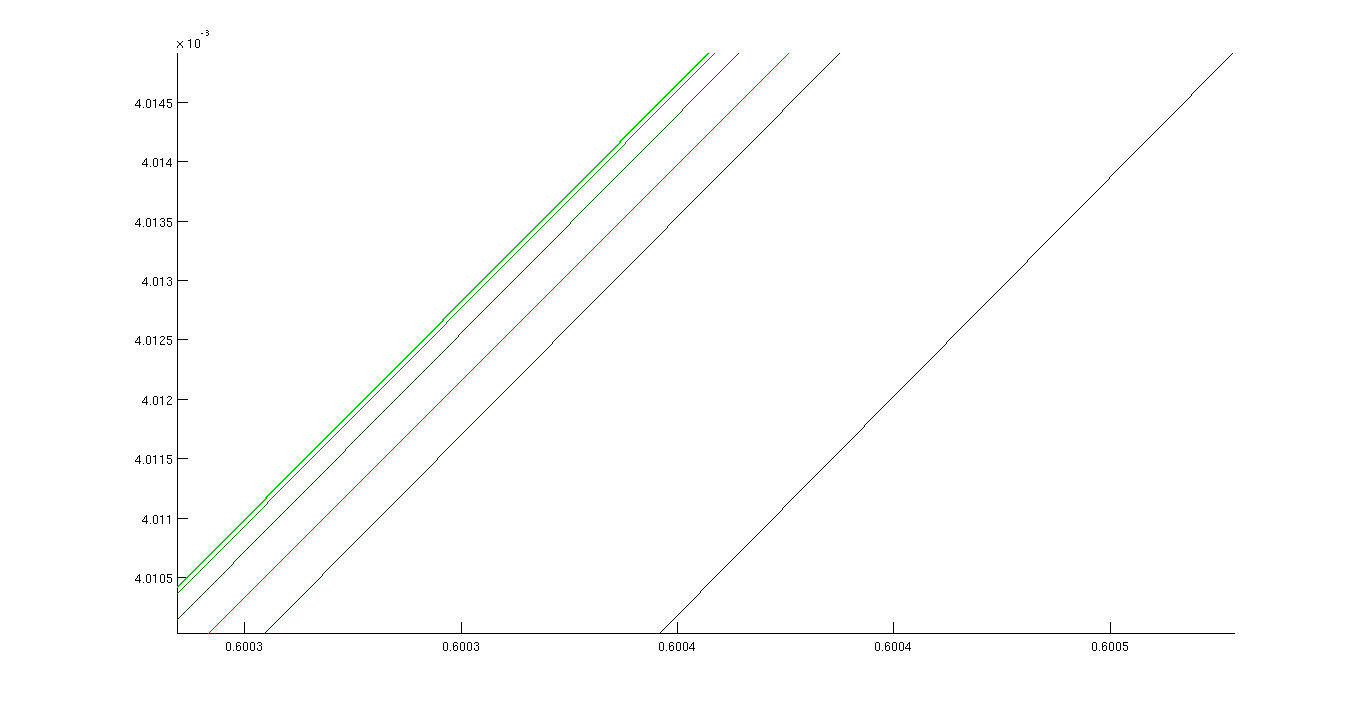
\includegraphics[width=\textwidth]{fig/azoom.png}
          \caption{One zooming}\label{fig:zooming}
        \end{subfigure}
        \caption{Plots of $u(x)$. The red line is the actual function.
        The others are estimations. The greener the line the higher
      $n$.}\label{fig:plots}
\end{figure}


\section{Table example}

\begin{table}[h]
  \begin{tabular}{r|c|c|c|}
    \multicolumn{1}{r}{}
     & \multicolumn{1}{c}{$Q_{classic}$ }
     & \multicolumn{1}{c}{$Q_{stable}$}
     & \multicolumn{1}{c}{$Q_{householder}$} \\
    \cline{2-4}
    $n=100$ & \input{data/norm-q-classi-100.dat}
            & \input{data/norm-q-stable-100.dat}
            & \input{data/norm-q-househ-100.dat}
            \\ \cline{2-4}
    $n=150$ & \input{data/norm-q-classi-150.dat}
            & \input{data/norm-q-stable-150.dat}
            & \input{data/norm-q-househ-150.dat}
            \\ \cline{2-4}
  \end{tabular}
  \caption{Norms for the different unitary $Q$ matrices}
  \label{tab:norms}
\end{table}

\begin{table}[h]
  \begin{tabular}{r|c|c|c|}
    \multicolumn{1}{r}{}
     & \multicolumn{1}{c}{$Q_{classic}$ }
     & \multicolumn{1}{c}{$Q_{stable}$}
     & \multicolumn{1}{c}{$Q_{householder}$} \\
    \cline{2-4}
    $n=100$ & \input{data/std-q-classi-100.dat}
            & \input{data/std-q-stable-100.dat}
            & \input{data/std-q-househ-100.dat}
            \\ \cline{2-4}
    $n=150$ & \input{data/std-q-classi-150.dat}
            & \input{data/std-q-stable-150.dat}
            & \input{data/std-q-househ-150.dat}
            \\ \cline{2-4}
  \end{tabular}
  \caption{The standard deviation for the values of $A-QR$}
  \label{tab:stds}
\end{table}

\newcommand{\genfig}[3] {{
    \begin{figure}
            \centering
            \begin{subfigure}[b]{1.0\textwidth}
                    \includegraphics[width=\textwidth]{fig/#1-#2-100}
                    \caption{$n = 100$}
            \end{subfigure}
            \begin{subfigure}[b]{1.0\textwidth}
                    \includegraphics[width=\textwidth]{fig/#1-#2-150}
                    \caption{$n = 150$}
            \end{subfigure}
            \caption{Medians of the columns of $\Delta #2$ #3}\label{fig:#1-#2}
    \end{figure}
  }}

\genfig{log-median-col}{Q}{logarithmized}
\genfig{median-row}{Q}{}
\genfig{log-median-col}{R}{logarithmized}
\genfig{log-median-row}{R}{logarithmized}


\end{document}
